\hypertarget{the-falicov-kimball-model}{%
\section{The Falicov Kimball Model}\label{the-falicov-kimball-model}}

\hypertarget{the-model}{%
\subsection{The Model}\label{the-model}}

\hypertarget{fig:simple_DOS}{%
\begin{figure}
\centering
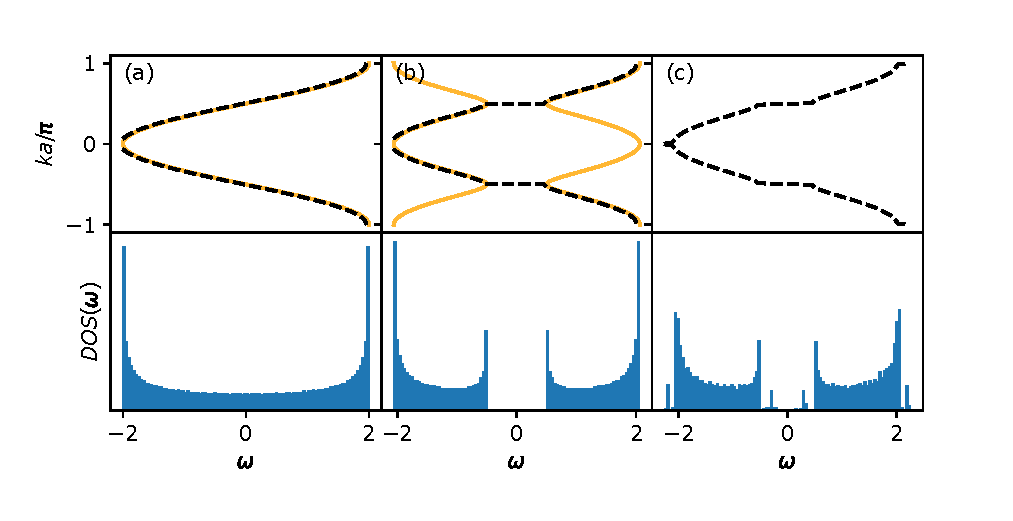
\includegraphics[width=1\textwidth,height=\textheight]{figure_code/background_chapter/simple_DOS}
\caption[{Cubic Lattice dispersion with disorder}]{The dispersion (upper row) and density of states (lower row) obtained from a cubic lattice model \(H = \sum_{i} V_i c^\dagger_{i}c^{\phantom{\dagger}}_{i} - t \sum_{\langle i,j\rangle} c^\dagger_{i}c^{\phantom{\dagger}}_{j}\) in 1D. (a) With no external potential. (b) With a static charge density wave background \(V_i = (-1)^i\) (c) A static charge density wave background with 2\% binary disorder. The top row shows the analytic dispersion in orange compared with the integral of the DOS in dotted black.}
\label{fig:simple_DOS}
\end{figure}
}

The Falicov-Kimball (FK) model is one of the simplest models of the correlated electron problem. It captures the essence of the interaction between itinerant and localised electrons. It was originally introduced to explain the metal-insulator transition in f-electron systems. However, in its long history, the FK model has been interpreted variously as a model of electrons and ions, binary alloys or crystal formation~\autocite{hubbardj.ElectronCorrelationsNarrow1963,falicovSimpleModelSemiconductorMetal1969,gruberFalicovKimballModelReview1996,gruberFalicovKimballModel2006}. In terms of immobile fermions \(d_i\) and light fermions \(c_i\) and with chemical potential fixed at half-filling, the model reads

\[\begin{aligned}
H_{\mathrm{FK}} = & \;U \sum_{i} (d^\dagger_{i}d_{i} - \tfrac{1}{2})\;(c^\dagger_{i}c^{\phantom{\dagger}}_{i} - \tfrac{1}{2}) -\;t \sum_{\langle i,j\rangle} c^\dagger_{i}c^{\phantom{\dagger}}_{j}.\\ 
\end{aligned}\]

Here we will only discuss the hypercubic lattices, i.e.,~the chain, the square lattice, the cubic lattice and so on. The connection to the Hubbard model is that we have relabelled the up and down spin electron states and removed the hopping term for one spin state. This is equivalent to taking the limit of infinite mass ratio~\autocite{devriesSimplifiedHubbardModel1993}.

Like other exactly solvable models~\autocite{smithDisorderFreeLocalization2017}, the FK model possesses extensively many conserved degrees of freedom \([d^\dagger_{i}d_{i}, H] = 0\). Similarly, the Kitaev model contains an extensive number of conserved fluxes. So in both models, the Hilbert space breaks up into a set of sectors in which these operators take a definite value. Crucially, this reduces the interaction terms in the model from being quartic in fermion operators to quadratic. This is what makes the two models exactly solvable, in contrast to the Hubbard model. For the FK model the interaction term \((d^\dagger_{i}d_{i} - \tfrac{1}{2})\;(c^\dagger_{i}c^{\phantom{\dagger}}_{i} - \tfrac{1}{2})\) becomes quadratic when \(d^\dagger_{i}d_{i}\) is replaced with one of its eigenvalues \(\{0,1\}\). The same thing happens in the Kitaev model, though after first applying a clever transformation which we will discuss later.

Due to Pauli exclusion, maximum filling occurs when each lattice site is fully occupied, \(\langle n_c + n_d \rangle = 2\). Here we will focus on the half-filled case \(\langle n_c + n_d \rangle = 1\). The ground state phenomenology as the model is doped away from the half-filled state can be rich~\autocite{jedrzejewskiFalicovKimballModels2001,gruberGroundStatesSpinless1990} but the half-filled point has symmetries that make it particularly interesting. From this point on, we will only consider the half-filled point.

At half-filling and on bipartite lattices, the FK model is particle-hole symmetric. That is, the Hamiltonian anticommutes with the particle hole operator \(\mathcal{P}H\mathcal{P}^{-1} = -H\). As a consequence, the energy spectrum is symmetric about \(E = 0\), which is the Fermi energy. \Cref{fig:simple_DOS} shows this in action, in the presence of a periodic potential a gap in the energy spectrum opens symmetrically about \(E = 0\). The particle hole operator corresponds to the substitution \(c^\dagger_i \rightarrow \epsilon_i c_i, d^\dagger_i \rightarrow d_i\) where \(\epsilon_i = +1\) for the A sublattice and \(-1\) for the B sublattice~\autocite{gruberFalicovKimballModel2006}. The absence of a hopping term for the heavy electrons means they do not need the factor of \(\epsilon_i\) but they would need it in the corresponding Hubbard model. See appendix \protect\hyperlink{particle-hole-symmetry}{A.1} for a full derivation of the particle-hole symmetry.

We will later add a long-range interaction between the localised electrons. At that point we will replace the immobile fermions with a classical Ising field \(S_i = \tfrac{1}{2}(1 - 2d^\dagger_id_i) = \pm\tfrac{1}{2}\) which I will refer to as the spins.

\[\begin{aligned}
H_{\mathrm{FK}} = & \;U \sum_{i} S_i\;(c^\dagger_{i}c^{\phantom{\dagger}}_{i} - \tfrac{1}{2}) -\;t \sum_{\langle i,j\rangle} c^\dagger_{i}c^{\phantom{\dagger}}_{j}.\\ 
\end{aligned}\]

The FK model can be solved exactly with dynamic mean field theory in the infinite dimensional limit~\autocite{antipovCriticalExponentsStrongly2014,ribicNonlocalCorrelationsSpectral2016,freericksExactDynamicalMeanfield2003,herrmannNonequilibriumDynamicalCluster2016}. In lower dimensional systems it has radically different behaviour, as we shall see.

\hypertarget{phase-diagrams}{%
\subsection{Phase Diagrams}\label{phase-diagrams}}

\hypertarget{fig:fk_phase_diagram}{%
\begin{figure}
\centering
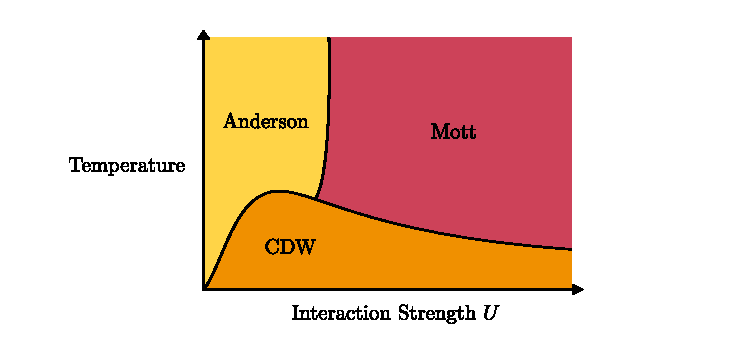
\includegraphics[width=1\textwidth,height=\textheight]{figure_code/background_chapter/fk_phase_diagram}
\caption[{Falicov-Kimball Temperature-Interaction Phase Diagrams}]{Schematic Phase diagram of the Falicov-Kimball model in dimensions two or more At low temperature the classical fermions (spins) settle into an ordered charge density wave state (antiferromagnetic state). The schematic diagram for the Hubbard model is the same. Reproduced from~\autocite{antipovInteractionTunedAndersonMott2016,antipovCriticalExponentsStrongly2014}.}
\label{fig:fk_phase_diagram}
\end{figure}
}

In dimensions greater than one, the FK model exhibits a phase transition at some \(U\) dependent critical temperature \(T_c(U)\) to a low temperature ordered phase~\autocite{maskaThermodynamicsTwodimensionalFalicovKimball2006}. In terms of the heavy electrons this corresponds to them occupying only one of the two sublattices A and B, known as a Charge Density Wave (CDW) phase. In terms of spins, this is an antiferromagnetic phase.

In the disordered region above \(T_c(U)\), there are two insulating phases. For weak interactions \(U << t\), thermal fluctuations in the spins act as an effective disorder potential for the fermions. This causes them to localise, giving rise to an Anderson insulating (AI) phase~\autocite{andersonAbsenceDiffusionCertain1958} which we will discuss more in section~\protect\hyperlink{bg-disorder-and-localisation}{2.3}. For strong interactions \(U >> t\), the spins are not ordered. Nevertheless, their interaction with the electrons opens a gap, leading to a Mott insulator analogous to that of the Hubbard model~\autocite{brandtThermodynamicsCorrelationFunctions1989}. The presence of an interaction driven phase like the Mott insulator in an exactly solvable model is part of what makes the FK model such an interesting system.

By contrast, in the 1D FK model there is no Finite-Temperature Phase Transition (FTPT) to an ordered CDW phase~\autocite{liebAbsenceMottTransition1968}. Indeed, dimensionality is crucial for the physics of both localisation and FTPTs. In 1D, disorder generally dominates: even the weakest disorder exponentially localises \emph{all} single particle eigenstates. In the 1D FK model, this means that the whole spectrum is localised at all finite temperatures~\autocite{goldshteinPurePointSpectrum1977,abrahamsScalingTheoryLocalization1979,kramerLocalizationTheoryExperiment1993}. Although at low temperatures, the localisation length may be so large that the states appear extended in finite sized systems~\autocite{antipovInteractionTunedAndersonMott2016}. Only longer-range correlations of the disorder potential can potentially induce localisation-delocalisation transitions in 1D~\autocite{aubryAnalyticityBreakingAnderson1980,dassarmaLocalizationMobilityEdges1990,dunlapAbsenceLocalizationRandomdimer1990}.

The absence of finite temperature ordered phases in 1D systems is a general feature. It can be understood as a consequence of the fact that domain walls are energetically cheap in 1D. Thermodynamically, short-range interactions just cannot overcome the entropy of thermal defects in 1D. However, the addition of longer range interactions can overcome this~\autocite{peierlsIsingModelFerromagnetism1936,kennedyItinerantElectronModel1986}.

The absence of an FTPT in the short ranged FK chain is far from obvious because the Ruderman-Kittel-Kasuya-Yosida (RKKY) interaction mediated by the fermions~\autocite{kasuyaTheoryMetallicFerro1956,rudermanIndirectExchangeCoupling1954,vanvleckNoteInteractionsSpins1962,yosidaMagneticPropertiesCuMn1957} decays as \(r^{-1}\) in 1D~\autocite{rusinCalculationRKKYRange2017}. This could, in principle, induce the necessary long-range interactions for the classical Ising background to order at low temperatures~\autocite{thoulessLongRangeOrderOneDimensional1969,peierlsIsingModelFerromagnetism1936}. However, Kennedy and Lieb established rigorously that, at half-filling, a CDW phase only exists at \(T = 0\) for the 1D FK model~\autocite{kennedyItinerantElectronModel1986}.

The 1D FK model has been studied numerically, perturbatively in interaction strength \(U\) and in the continuum limit~\autocite{bursillOneDimensionalContinuum1994}. The main results are that for attractive \(U > U_c\) the system forms electron spin bound state `atoms' which repel one another~\autocite{gruberGroundStateEnergyLowTemperature1993} and that the ground state phase diagram has a fractal structure as a function of electron filling, a devil's staircase~\autocite{freericksTwostateOnedimensionalSpinless1990,michelettiCompleteDevilStaircase1997}.

Based on this primacy of dimensionality, we will go digging into the 1D case. In chapter~\protect\hyperlink{chap:3-the-long-range-falicov-kimball-model}{3}, we will construct a generalised 1D FK model with long-range interactions, which induces the otherwise forbidden CDW phase at non-zero temperature. To do this, we will draw on theory of the Long-Range Ising (LRI) model which is the subject of the next section.

\hypertarget{long-ranged-ising-model}{%
\subsection{Long-Ranged Ising model}\label{long-ranged-ising-model}}

The suppression of phase transitions is a common phenomenon in 1D systems and the Ising model serves as the canonical illustration of this. In terms of classical spins \(S_i = \pm 1\) the standard Ising model reads

\[H_{\mathrm{I}} = \sum_{\langle ij \rangle} S_i S_j.\]

Like the FK model, the Ising model shows an FTPT to an ordered state only in 2D and above. This can be understood via Peierls' argument~\autocite{peierlsIsingModelFerromagnetism1936,kennedyItinerantElectronModel1986} to be a consequence of the low energy penalty for domain walls in 1D systems.

\hypertarget{fig:ising_model_domain_wall}{%
\begin{figure}
\centering
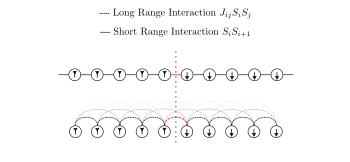
\includegraphics[width=1\textwidth,height=\textheight]{figure_code/intro_chapter/ising_model_domain_wall}
\caption[{Domain walls in the long-range Ising Model}]{Domain walls in the 1D Ising model cost finite energy because they affect only one interaction. In the Long-Range Ising (LRI) model it depends on how the interactions decay with distance.}
\label{fig:ising_model_domain_wall}
\end{figure}
}

Following Peierls' argument, consider the difference in free energy \(\Delta F = \Delta E - T\Delta S\) between an ordered state and a state with single domain wall as in \cref{fig:ising_model_domain_wall}. If this value is negative, it implies that the ordered state is unstable with respect to domain wall defects, and they will thus proliferate, destroying the ordered phase. If we consider the scaling of the two terms with system size \(L\), we see that short range interactions produce a constant energy penalty \(\Delta E\) for a domain wall. In contrast, the number of such single domain wall states scales linearly with system size so the entropy is \(\propto \ln L\). Thus, the entropic contribution dominates (eventually) in the thermodynamic limit and no finite temperature order is possible. In 2D and above, the energy penalty of a large domain wall scales like \(L^{d-1}\) which is why they can support ordered phases. This argument does not quite apply to the FK model because of the aforementioned RKKY interaction. Instead, this argument will give us insight into how to recover an ordered phase in the 1D FK model.

\hypertarget{fig:alpha_diagram}{%
\begin{figure}
\centering
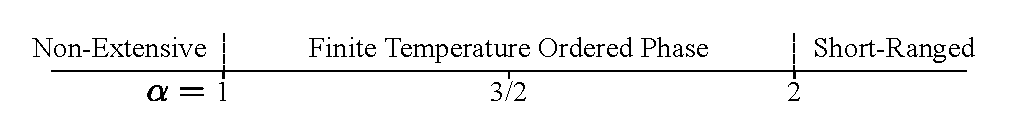
\includegraphics[width=1\textwidth,height=\textheight]{figure_code/background_chapter/alpha_diagram}
\caption[{Long-Range Ising Model Behaviour}]{The thermodynamic behaviour of the long-range Ising model \(H_{\mathrm{LRI}} = J \sum_{i\neq j} |i - j|^{-\alpha} S_i S_j\) as the exponent of the interaction \(\alpha\) is varied. In my simulations I stick to a value of \(\alpha = \tfrac{5}{4}\) to avoid the complexity of non-universal critical exponents that arise above \(\alpha = \tfrac{3}{2}\)}
\label{fig:alpha_diagram}
\end{figure}
}

In contrast, the LRI model \(H_{\mathrm{LRI}}\) can have an FTPT in 1D.

\[H_{\mathrm{LRI}} = \sum_{ij} J(|i-j|) S_i S_j = J \sum_{i\neq j} |i - j|^{-\alpha} S_i S_j.\]

Renormalisation group analyses show that the LRI model has an ordered phase in 1D for \(1 < \alpha < 2\) ~\autocite{dysonExistencePhasetransitionOnedimensional1969}. Peierls' argument can be extended~\autocite{thoulessLongRangeOrderOneDimensional1969} to long-range interactions to provide intuition for why this is the case. Let's consider again the energy difference between the ordered state \(|\ldots\uparrow\uparrow\uparrow\uparrow\ldots\rangle\) and a domain wall state \(|\ldots\uparrow\uparrow\downarrow\downarrow\ldots\rangle\). In the case of the LRI model, careful counting shows that this energy penalty is \begin{equation}\protect\hypertarget{eq:bg-dw-penalty}{}{\Delta E \propto \sum_{n=1}^{\infty} n J(n),}\label{eq:bg-dw-penalty}\end{equation}

because each interaction between spins separated across the domain by a bond length \(n\) can be drawn between \(n\) equivalent pairs of sites. The behaviour then depends crucially on how \cref{eq:bg-dw-penalty} scales with system size. Ruelle proved rigorously for a very general class of 1D systems that if \(\Delta E\) or its many-body generalisation converges to a constant in the thermodynamic limit then the free energy is analytic~\autocite{ruelleStatisticalMechanicsOnedimensional1968}. This rules out a finite order phase transition, though not one of the Kosterlitz-Thouless type. Dyson also proved this, though with a slightly different condition on \(J(n)\)~\autocite{dysonExistencePhasetransitionOnedimensional1969}.

With a power law form for \(J(n)\), there are a few cases to consider: For \(\alpha = 0\) i.e., infinite range interactions, the Ising model is exactly solvable and mean field theory is exact~\autocite{lipkinValidityManybodyApproximation1965}. This limit is the same as the infinite dimensional limit. For \(\alpha \leq 1\) we have very slowly decaying interactions. \(\Delta E\) does not converge as a function of system size so the Hamiltonian is non-extensive, a topic not without some considerable controversy~\autocite{grossNonextensiveHamiltonianSystems2002,lutskoQuestioningValidityNonextensive2011,wangCommentNonextensiveHamiltonian2003} that I will not consider further here. For \(1 < \alpha < 2\), we get a phase transition to an ordered state at a finite temperature. This is what we want! At the special point \(\alpha = 2\), the energy of domain walls diverges logarithmically. This turns out to be a Kostelitz-Thouless transition~\autocite{thoulessLongRangeOrderOneDimensional1969}. Finally, for \(\alpha > 2\) we have very quickly decaying interactions and domain walls again have a finite energy penalty. Hence, Peirels' argument holds and there is no phase transition.

One final complexity is that for \(\tfrac{3}{2} < \alpha < 2\) renormalisation group methods show that the critical point has non-universal critical exponents that depend on \(\alpha\) ~\autocite{fisherCriticalExponentsLongRange1972}. To avoid this potential confounding factor we will park ourselves at \(\alpha = 1.25\) when we apply these ideas to the FK model.

Were we to extend this to arbitrary dimension \(d\), we would find that, in general, both \(d\) and \(\alpha\) affect the thermodynamic properties of the model. Long-range interactions essentially modify the `effective dimension' of thermodynamic system~\autocite{angeliniRelationsShortrangeLongrange2014}.
